\section{Algorithm}
The MM trigger processor algorithm used is fully described in Ref. \cite{tpsim}. For briefness, we assume the diligent reader has familiarized themself withe new algorithm. 
\par Our implementation has 12-strip roads, staggered by 8 strips. The firmware implemented for the Harvard Micromegas octuplet is a single TPR containing 64 X roads. For each X road we have 9 overlapping stereo diamonds, shown in Fig. \ref{fig:diamonds}, two of which cover a redundant region but remain an artifact of the firmware. Nathan is working very hard to remove this.
\par A trigger track is required to have 3 X planes and 3 U,V planes. The ART time collection window spans 8 BCs. The first stage of the finder can process at most two 4-level X roads, and the second stage of the finder can process at most 3 triggers per X road (check this).
\par There are also built-in offsets into the VMM channel decoding which limit the fiducial region to 0 to 179.2 mm in x (the precision coordinate). When studying the efficiency, a fiducial cut is applied.

\begin{figure}[!htpb]
  \begin{center}
    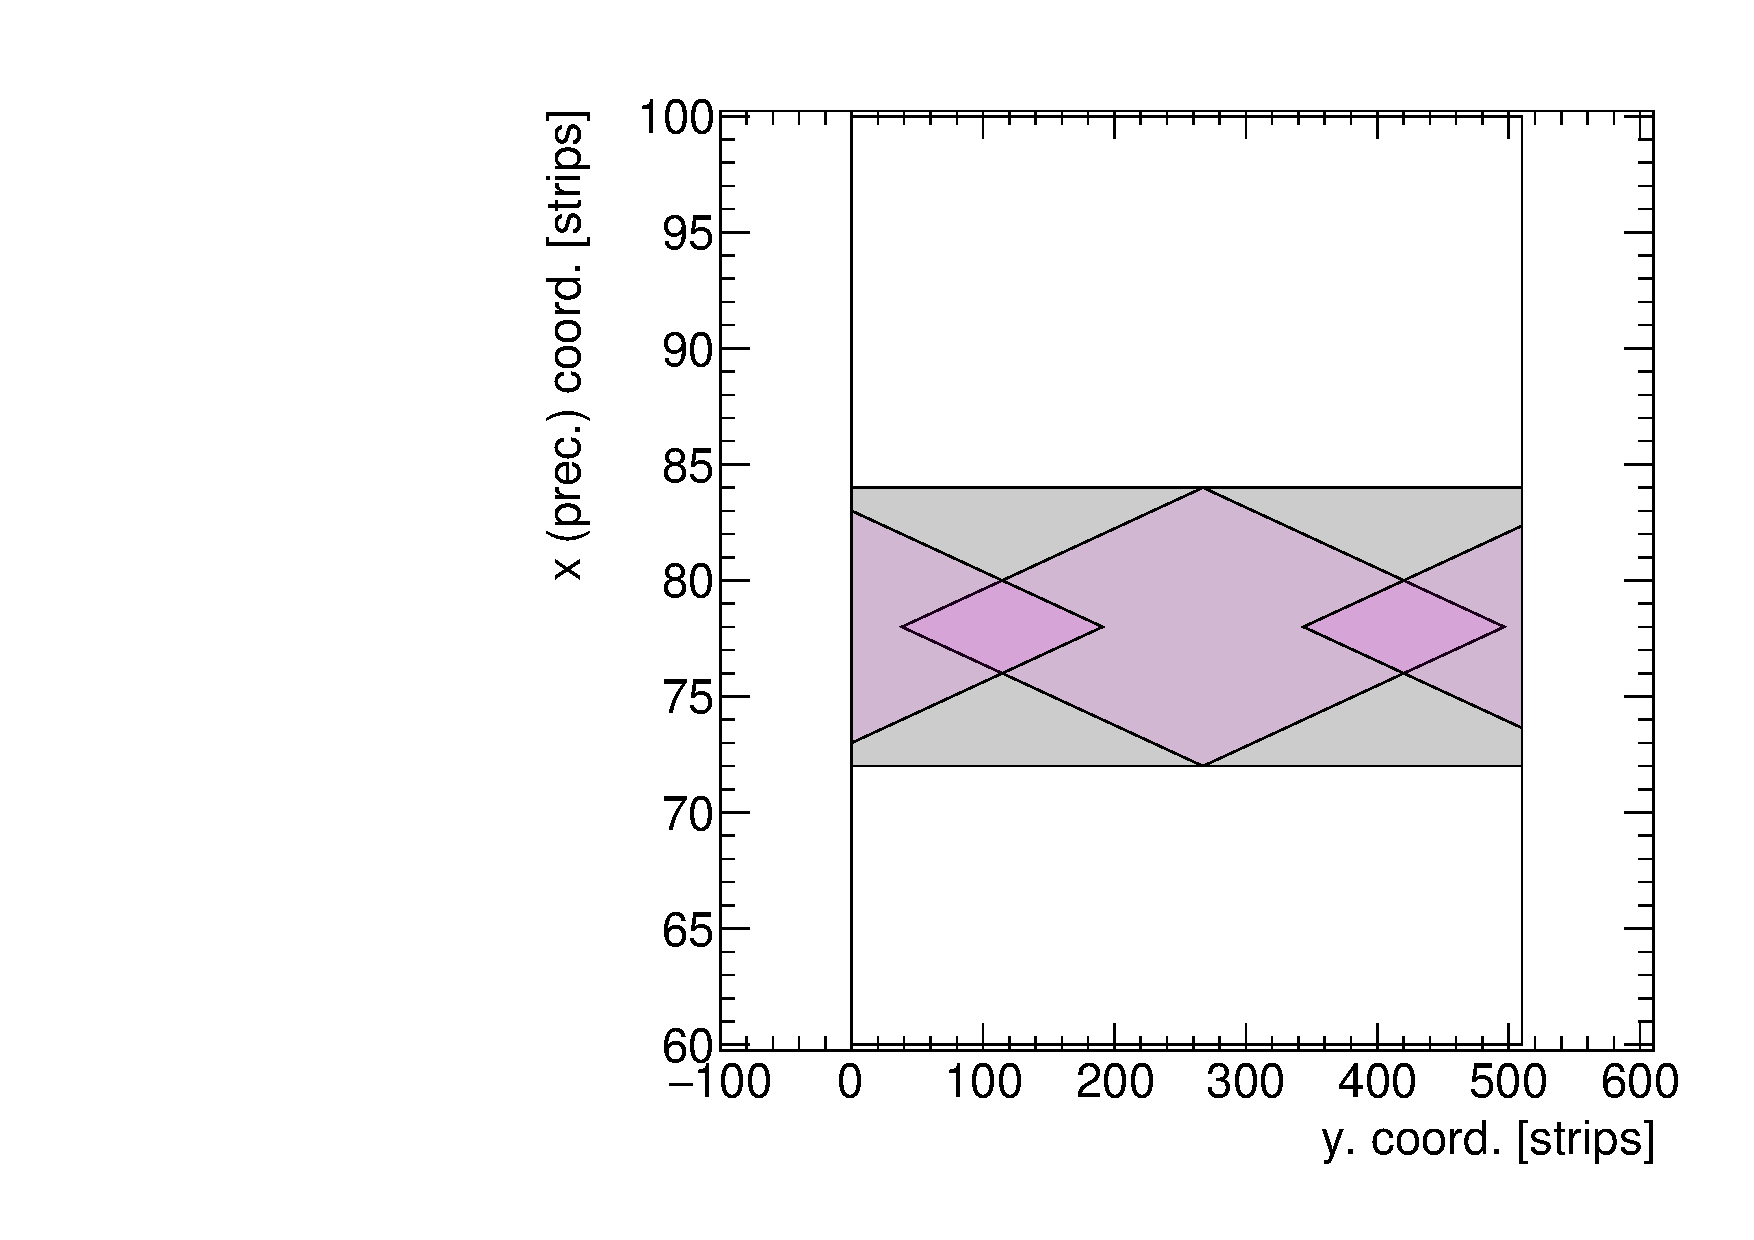
\includegraphics[width=0.3\textwidth]{figures/plot_horiz.pdf}
    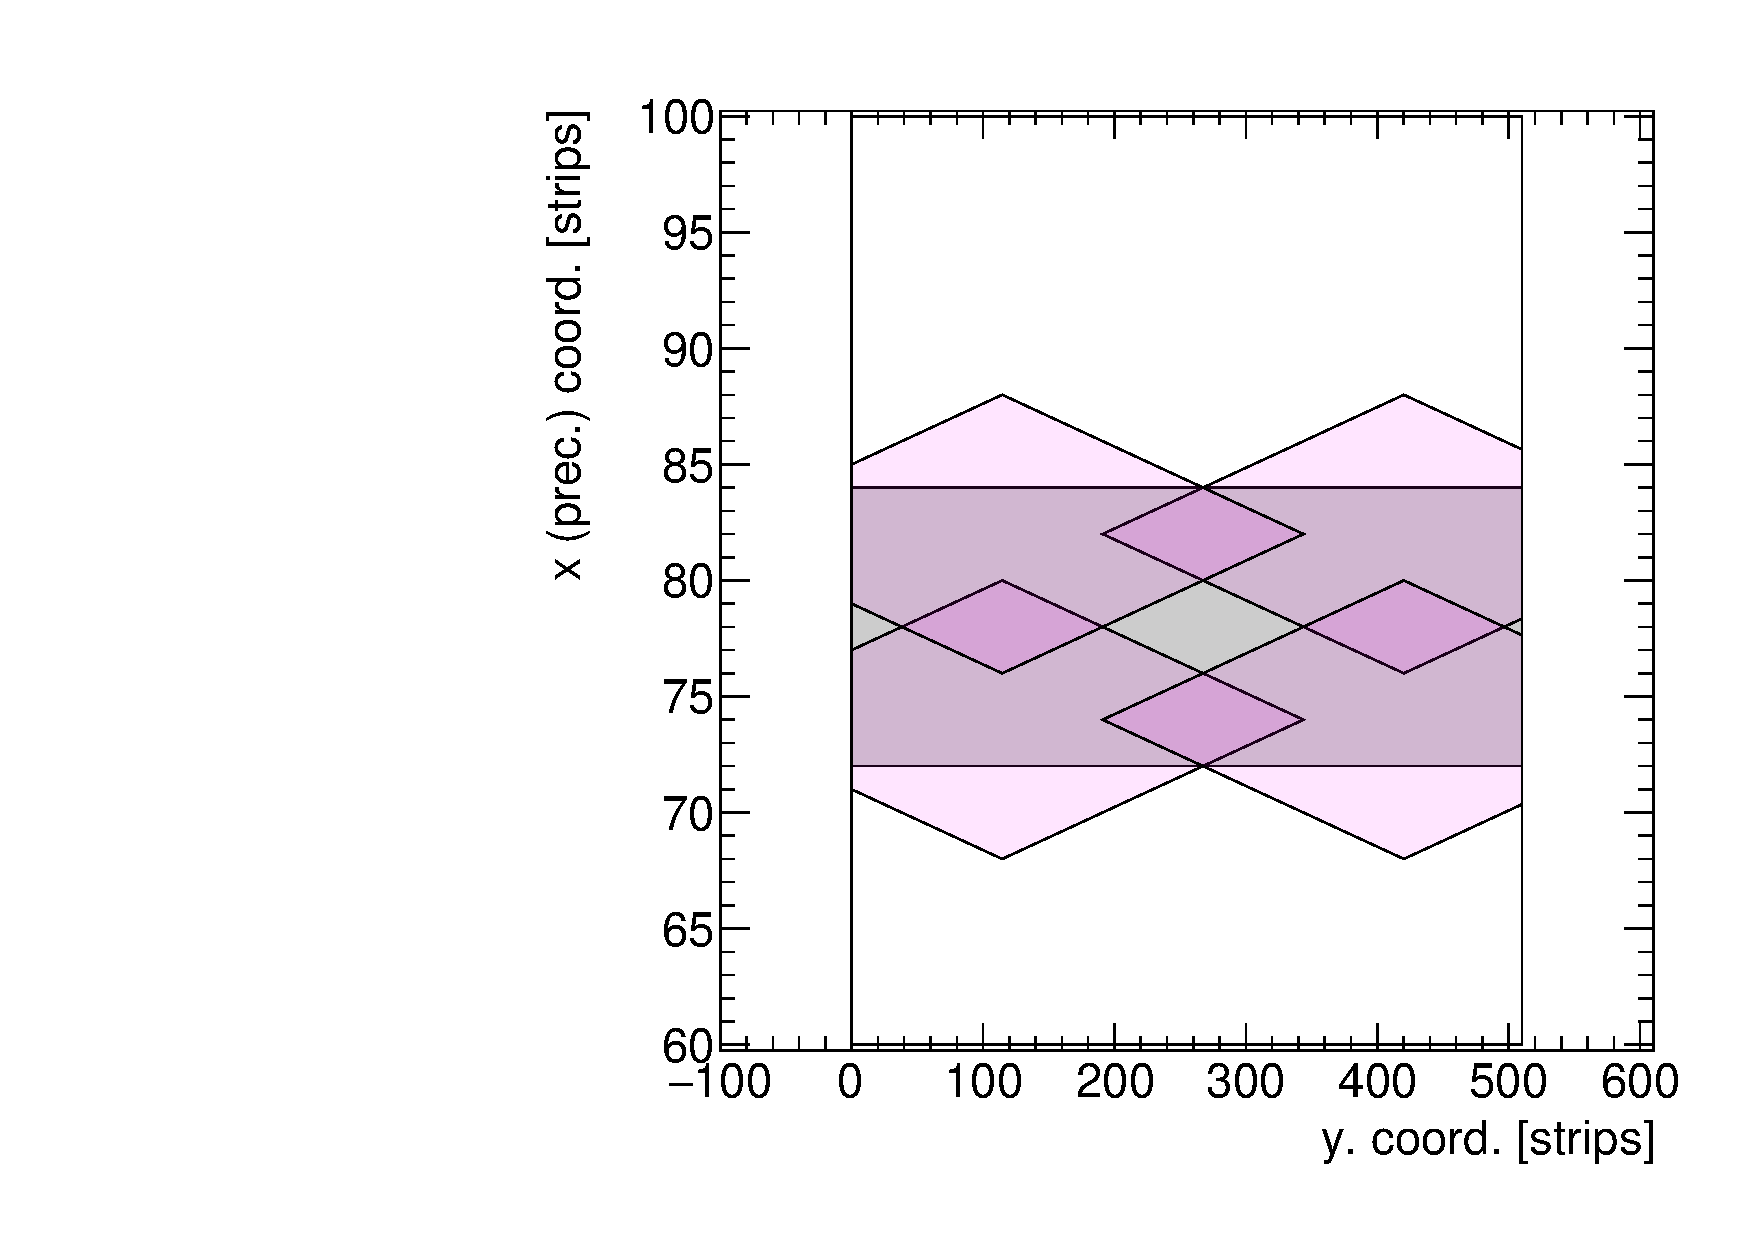
\includegraphics[width=0.3\textwidth]{figures/plot_surround.pdf}
    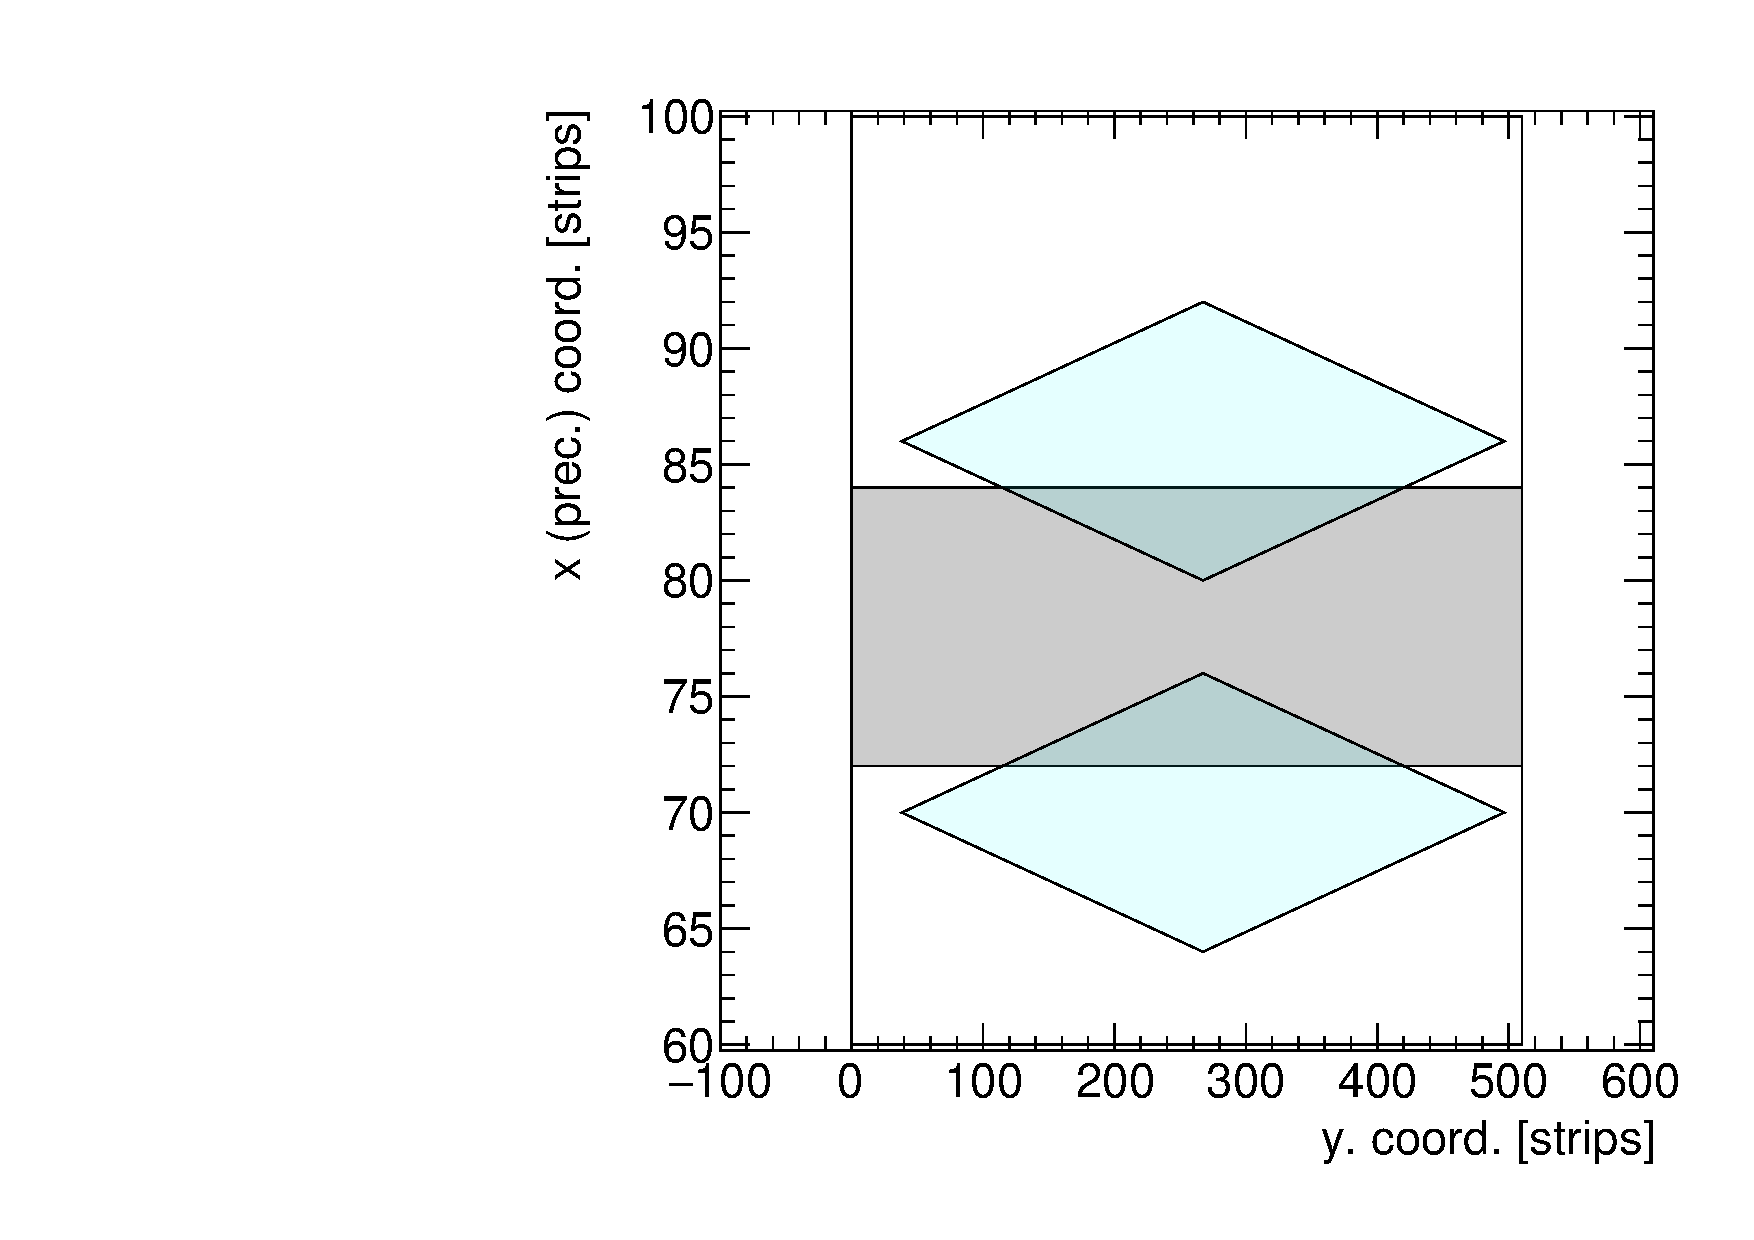
\includegraphics[width=0.3\textwidth]{figures/plot_extra.pdf}
  \end{center}
  \vspace{-10pt}
  \caption{The associated diamonds implemented for a single X-road (grey) are shown in pink and blue. The blue diamonds are redundant with the region covered by the pink diamonds.}
  \label{fig:diamonds}
\end{figure}



